%% chapters/behavior_modeling/ch2_rut.tex
%% 第2章　ランダム効用最大化理論の基礎

\section{ランダム効用最大化理論}\label{sec:abms}

本節では行動モデルの理解にあたり，ランダム効用最大化理論（Random Utility Maximization Theory, RUT）を導入する．
RUT はミクロ経済学の重要な仮定であり，個人は効用を最大化するような合理的な選択行動を行うとするものである．

\subsection{効用の記述とランダム性の導入}
まず選択肢の効用評価の記述方法を述べる．
各選択肢 $a$ は分析者によって設定された説明変数 $x_{i}$ および対応するパラメータ $\beta_{i}$ を用いて評価される．
その評価関数を効用関数と呼び，通常は線形な形式で表される．
すなわち，選択肢 $a$ の効用 $U_{a}$ は以下のように表される．
\begin{equation}\label{eq:utility_func_det}
U_{a} = \sum_{i} \beta_{i} x_{i}
\end{equation}
なお本定式化では個人の異質性は考慮していない．
例えば交通手段選択であれば，説明変数 $\bm{x}$ は「旅行時間」「旅行費用」「快適さ」などの属性を表し，パラメータ $\bm{\beta}$ はこれらの属性が効用に与える影響の大きさを表す．
行動モデルの目的は，この効用関数を用いて個人の選択行動を記述することであり，それは各パタメータ $\beta_{i}$ を推定することに帰着する．

個人 $k$ の選択行動結果を $y_k$ と表すと，効用最大化の仮定により
\begin{equation}\label{eq:utility_max}
y_k = \argmax_{a} U_{a}
\end{equation}
となる．
これは毎回確定的な選択が行われることを示すが，現実の選択行動は個人の置かれた状況に応じて変動することが予想される．
また\eqref{eq:utility_func_det}は各選択肢が分析者によって選定された特定の説明変数 $\bm{x}$ に基づいて評価されることを前提としているが，実際には分析者が行動に影響を与える全ての説明変数を把握することは困難である．
このような不確実性を考慮するために，効用関数\eqref{eq:utility_func_det}にランダムな誤差項 $\varepsilon_a$ を導入する．
すなわち，選択肢 $a$ の効用は以下のように再定義される．
\begin{equation}\label{eq:utility_func_random}
U_{a} = \sum_{i} \beta_{i} x_{a, i} + \varepsilon_a
\end{equation}
$\varepsilon_a$ は選択肢 $a$ に特有のランダムな誤差項であり，上で述べた個人の選択行動に影響を与えるが分析者が観測できない要因を表す．
なおこの誤差項に対し，従来の確定的な効用項 $V_a = \sum_i \beta_i x_{a, i}$ を確定項と呼ぶ．

\subsection{誤差項の分布に関する仮定}
誤差項によるランダム性の導入に伴い，\eqref{eq:utility_max}は次のように書き換えられる．
\begin{equation}\label{eq:utility_max_random}
y_k = \argmax_{a} \left( \sum_{i} \beta_{i} x_{a, i} + \varepsilon_a \right) = \argmax_{a} \left( V_a + \varepsilon_a \right)
\end{equation}
よって選択肢 $a$ の選択確率は次のように表される．
\begin{equation}
  \begin{aligned}
    \text{Pr}(y_k = a) &= \text{Pr}\left( V_a + \varepsilon_a > V_{a'} + \varepsilon_{a'} \quad \forall a' \neq a \right) \\
    &= \text{Pr}\left( V_a - V_{a'} > \varepsilon_{a'} - \varepsilon_a \quad \forall a' \neq a \right) \\
    &= \text{Pr}_{\varepsilon}\left( V_a - V_{a'} > \varepsilon \quad \forall a' \neq a \right) \\
    &= \int_{-\infty}^{V_a - V_{a'}} f(\varepsilon) d\varepsilon \\
    &= F_{\varepsilon}(V_a - V_{a'})
  \end{aligned}
\end{equation}

従って選択確率は誤差項 $\varepsilon$ の確率分布 $f(\varepsilon)$ および累積分布関数 $F_{\varepsilon}(\varepsilon)$ に明らかに依存する．

では続いてこの誤差項 $\varepsilon$ の分布形状を具体的に考えてみよう．

\subsubsection{正規分布の場合}
最も一般的な分布は正規分布である．
ここで標準正規分布の確率密度関数を $\phi(\cdot)$，その累積分布関数を $\Phi(\cdot)$ と表すと，選択確率 $\text{Pr}(y_k = a)$ は次のように表される．
\begin{equation}
  \text{Pr}(y_k = a) = \int_{-\infty}^{V_a - V_{a'}} \phi(\varepsilon) \, d\varepsilon = \Phi(V_a - V_{a'})
\end{equation}
この選択確率は一般に閉じた形で表すことができないため，数値的な積分が必要となる．
このモデルは Probit Modelと呼ばれる．

\subsubsection{Gumbel 分布の場合}
Gumbel 分布は正規分布と類似の形状を持つが，累積分布関数がclosed-formで表されるという特徴がある．
この分布を仮定すると，選択確率は次のように表される．
\begin{equation}
  \text{Pr}(y_k = a) = \frac{\exp(V_a)}
\end{equation}

\begin{figure}[hbtp]
  \centering
    \resizebox{.9\linewidth}{!}{%
      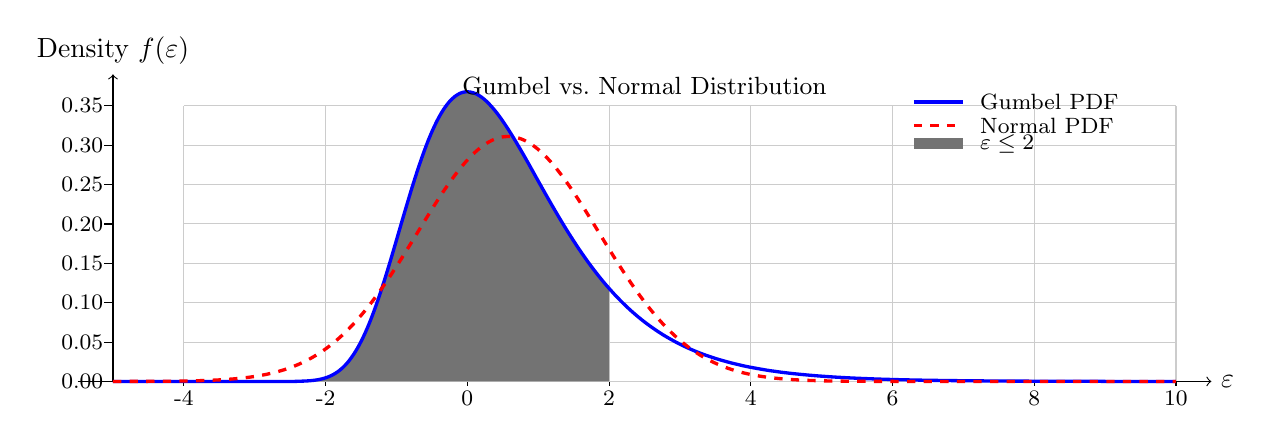
\begin{tikzpicture}[x=0.9cm,y=10cm]
  % axes
  \draw[->] (-5.5,0) -- (10.5,0) node[right] {$\varepsilon$};
  \draw[->] (-5,0) -- (-5,0.39) node[above] {Density $f(\varepsilon)$};

  % x ticks
  \foreach \x in {-4,-2,0,2,4,6,8,10}{
    \draw (\x,0) -- (\x,-0.006);
    \node[below,font=\footnotesize] at (\x,0) {\x};
  }

  % y ticks
  \foreach \y in {0.00,0.05,0.10,0.15,0.20,0.25,0.30,0.35}{
    \draw (-5,\y) -- (-5.12,\y);
    \node[left,font=\footnotesize] at (-5,\y) {\y};
  }

  % grid
  \draw[gray!40, thin] (-4,0) grid[xstep=2,ystep=0.05] (10,0.35);

  % shaded area
  \fill[black!55]
    plot[smooth,domain=-5:2,samples=120]
      (\x,{exp(-(\x + exp(-\x)))})
    -- (2,0) -- (-5,0) -- cycle;

  % Gumbel curve
  \draw[blue, very thick]
    plot[smooth,domain=-5:10,samples=200]
      (\x,{exp(-(\x + exp(-\x)))});

  % Normal distribution (mu=0.5772, sigma=pi/sqrt(6)=1.2826) to match Gumbel mean & variance
  \draw[red, very thick, dashed]
    plot[smooth,domain=-5:10,samples=200]
      (\x,{exp(-0.5*((\x - 0.5772)/1.2826)^2) / (1.2826*2.5066)});

  % title
  \node[font=\small] at (2.5,0.375)
    {Gumbel vs.\ Normal Distribution};

  % legend
  \draw[blue, very thick] (6.3,0.355) -- (7.0,0.355);
  \node[right,font=\footnotesize] at (7.1,0.355) {Gumbel PDF};

  \draw[red, very thick, dashed] (6.3,0.325) -- (7.0,0.325);
  \node[right,font=\footnotesize] at (7.1,0.325) {Normal PDF};

  \fill[black!55] (6.3,0.295) rectangle (7.0,0.309);
  \node[right,font=\footnotesize] at (7.1,0.302) {$\varepsilon \le 2$};
\end{tikzpicture}%
    }
  \caption{Gumbel 分布の確率密度関数(PDF)と，$\varepsilon \le 2$ の領域}
  \label{fig:gumbel-pdf}
\end{figure}

以降の議論では $\varepsilon_a$ の形状および独立同一性に関する仮定が重要な役割を果たすが，ここではまずランダム性の導入の意義を理解することに留める．

\subsubsection{独立同一性: Independent Identical Distribution (IID)}
\begin{description}
  \item[独立性] 各選択肢 $a$ に対して $\varepsilon_a$ は互いに独立である．
  \item[同一分布] 各選択肢 $a$ に対して $\varepsilon_a$ は同一の確率分布に従う．
\end{description}
この二つの仮定は，選択肢間の相関や個人の異質性を考慮しないことを意味する．




% 選択肢 $a$ は「自動車」「公共交通機関」「徒歩」などの交通手段であり，説明変数 $x_{i}$ は「旅行時間」「旅行費用」「快適さ」などの属性である．
% 効用 $U_{ai}$ を評価する：
% %% chapters/assignment/ch6_evogame.tex
% %% 第6章　進化ゲーム理論と交通配分（Sandholm 2010）

% \section{進化ゲーム理論と交通配分}
% \label{sec:ch6-evogame}

% \sref{sec:ch3-ue}では，利用者均衡配分（UE）が
% Beckmann 変換によって凸最適化問題（UE/FD-Primal）と等価であることを示し，
% Frank-Wolfe 法によって数値的に解けることを確認した\cite{Beckmann1956,Wardrop1952}．
% しかし，静学的な UE 分析が答えるのは「均衡状態がどこにあるか」という問いのみであり，
% 「利用者がどのようにして均衡に到達するか」という\textbf{ダイナミクス}の問いには答えない．

% 本節では，この問いに答えるための枠組みとして\textbf{進化ゲーム理論}を導入する
% \cite{Sandholm2010,Sandholm2001}．
% まず，UE がポテンシャルゲームの最小値と等価であるという静学的な関係を整理し
% （\ssref{subsec:potential-game}），
% この枠組みを進化的 Day-to-day ダイナミクスへ拡張する動機を説明する
% （\ssref{subsec:evo-game-overview}）．
% 続いて \textbf{集団ゲーム}（Population Game）の基本概念を導入し
% （\ssref{subsec:population-game}），
% 有限合理性のもとでの乗り換え行動を記述する
% \textbf{改訂プロトコル}（Revision Protocol）と
% \textbf{集団ダイナミクス}（Mean Dynamics）の理論的枠組みを示す
% （\ssref{subsec:revision-protocol}）．
% \ssref{subsec:dynamics-examples} では交通配分に関連する代表的な進化動学を紹介し，
% \ssref{subsec:stability-convergence} で収束定理を述べ，
% \ssref{subsec:daytodaydyn} で Day-to-day ダイナミクスの交通政策への含意を考察する．

% % ---------------------------------------------------------------
% \subsection{ポテンシャルゲームとしての UE}
% \label{subsec:potential-game}
% % ---------------------------------------------------------------

% \subsubsection*{ポテンシャルゲームの概念}

% UE の最適化問題（\ssref{subsec:beckmann}）を
% ゲーム理論の視点から捉え直すと，その背後に
% \textbf{ポテンシャルゲーム}（Potential Game）の構造が見えてくる
% \cite{Monderer1996}．

% ポテンシャルゲームとは，すべてのプレーヤーの「利得の変化」が，
% 1 つのグローバルな関数 $Q$（\textbf{ポテンシャル関数}）の変化に
% きっかりと等しいゲームである．
% すなわち，プレーヤー $a$ が戦略を $i$ から $j$ に変更したとき：